\begin{figure}[H]
    \centering
    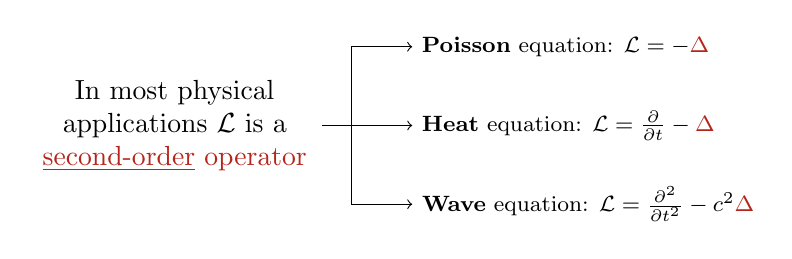
\begin{tikzpicture}
        \node[align=center,text width=3.5cm] at (0,0) (A) {In most physical applications $\mathcal{L}$ is a \textcolor{BrickRed}{\underline{second-order} operator}};

        \node at (5,0) (B) {\footnotesize{\textbf{Heat} equation: $\mathcal{L}=\frac{\partial}{\partial t}-\textcolor{BrickRed}{\Delta}$}};

        \node at (4.965,1) (C) {\footnotesize{\textbf{Poisson} equation: $\mathcal{L}=-\textcolor{BrickRed}{\Delta}$}};

        \node at (5.25,-1) (D) {\footnotesize{\textbf{Wave} equation: $\mathcal{L}=\frac{\partial^2}{\partial t^2}-c^2\textcolor{BrickRed}{\Delta}$}};

        \draw[->] (A) -- (B);
        \draw[->] (2.25,0) -- (2.25,1) -- (C);
        \draw[->] (2.25,0) -- (2.25,-1) -- (D); 
    \end{tikzpicture}
\end{figure}